% $Id: Grid_desc.tex,v 1.20 2006/01/10 17:44:31 jwolfe Exp $
%
% Earth System Modeling Framework
% Copyright 2002-2003, University Corporation for Atmospheric Research, 
% Massachusetts Institute of Technology, Geophysical Fluid Dynamics 
% Laboratory, University of Michigan, National Centers for Environmental 
% Prediction, Los Alamos National Laboratory, Argonne National Laboratory, 
% NASA Goddard Space Flight Center.
% Licensed under the GPL.

% <Describe class function and relation to other classes.>

The ESMF Grid class represents all aspects of the computational domain and its
decomposition in a parallel-processing environment, and must provide access to
any necessary grid information to the rest of the ESMF.  The ESMF Grid class
is included in the Field class and the Gridded Component class
and provides information needed in data communication methods like halo and
redistribution.  It has methods to internally generate a variety of
simple grids or read in more complicated grids provided by a user 
(reading in grids is not yet implemented).  The ESMF Grid class supports
multi-component coupling by providing a common structure necessary for regridding.

ESMF Grids are currently assumed to be two-dimensional, logically-rectangular
horizontal grids, with an optional vertical grid whose coordinates are
independent of those of the horizontal grid.  Each Grid is assigned a
staggering in its create method call, which helps define the Grid according
to typical Arakawa nomenclature.  The staggering of the Grid sets the possible
relative locations ({\tt ESMF\_Rellocs}) for the Fields associated with that
Grid.  This interaction between Grid and data placement is explained in detail
in Section~\ref{sec:GridDataPlacement}.

ESMF differentiates between global data, which describes a complete set of data,
and DE-local data, which describes a distributed or decomposed chuck of data
located on a single DE.  The Grid class plays an integral role in this concept.
A Grid is first instantiated, via a create call, on all DEs in its domain, but
only in a global sense.  By that we mean it stores only information about the
global Grid, such as the number of grid cells and the coordinate extents, but
has not generated all the information that will end up distributed, such as the
cell coordinates.  The Grid is then decomposed onto a given DELayout via an
{\tt ESMF\_Distribute()} call.  At that point, the DE-local data types are
created and computed, so that on each DE there resides necessary global Grid
information as well as its own DE-local Grid data.  The DE-local data represented
by an {\tt ESMF\_Field} is defined by the decomposition of the underlying
{\tt ESMF\_Grid}.

\subsubsection{Grids and Data Placement}
\label{sec:GridDataPlacement}
An {\tt ESMF\_Grid} will support data placement only at specific cell relative
locations, defined by its staggering and following typical Arakawa nomenclature.
In ESMF, there are nine possible relative locations for data on a typical
horizontal Grid cell, though each staggering will use a subset of them.  These
locations, with their corresponding {\tt ESMF\_Rellocs}, are illustrated in
% Figure~\ref{fig:GridDataLocations}.

% DIAGFIX_BASELINE6
% \begin{center}
% \begin{figure}[h!tb]
% \caption{Possible horizontal data locations for a representative computational
% cell. }
% \label{fig:GridDataLocations}
% \scalebox{0.66}{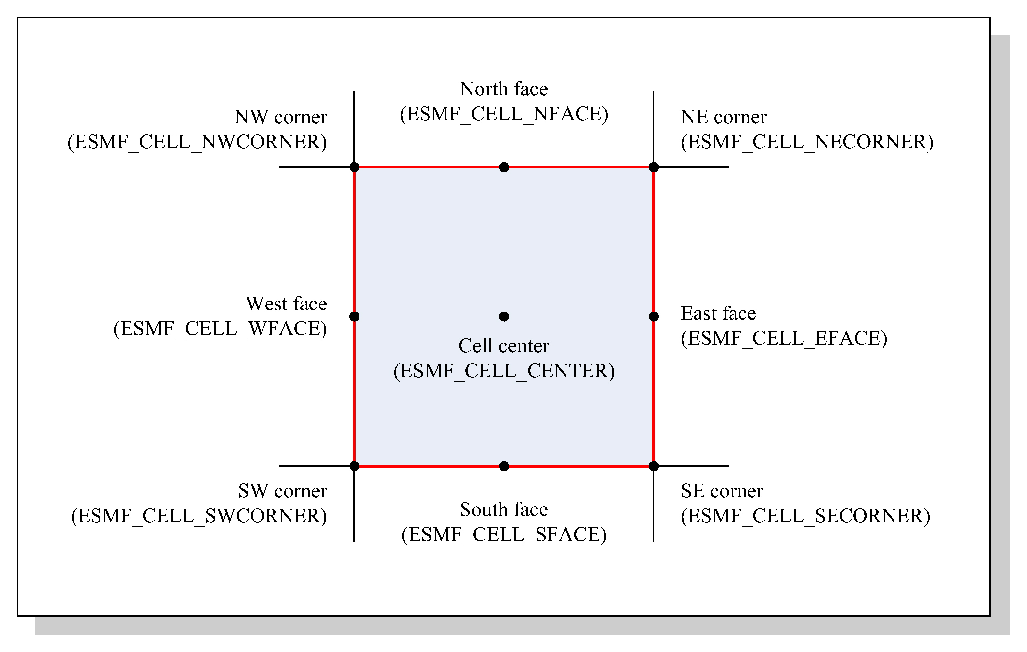
\includegraphics{GridDataLocations}}
% \end{figure}
% \end{center}

{\tt ESMF\_Grids} are created with only those underlying structures, called
subGrids, to support data at the specific cell locations defined by its given
staggering.  For example, an Arakawa C grid has some computational fields
defined at the cell centers and other fields defined at specific cell face
centers.  An {\tt ESMF\_Grid} created with Arakawa C staggering will therefore
make subGrids at the cell centers and specified cell faces (please see
Section~\ref{sec:GridHorzStagger} for a complete list of implemented staggerings
and their corresponding Rellocs).  An example of the data locations for an
% Arakawa C\_SE Grid is presented in Figure~\ref{fig:ArakawaC_SE}.

% DIAGFIX_BASELINE7
% \begin{center}
% \begin{figure}[h!tb]
% \caption{Data locations for an Arakawa C\_SE Grid. }
% \label{fig:ArakawaC_SE}
% \scalebox{0.66}{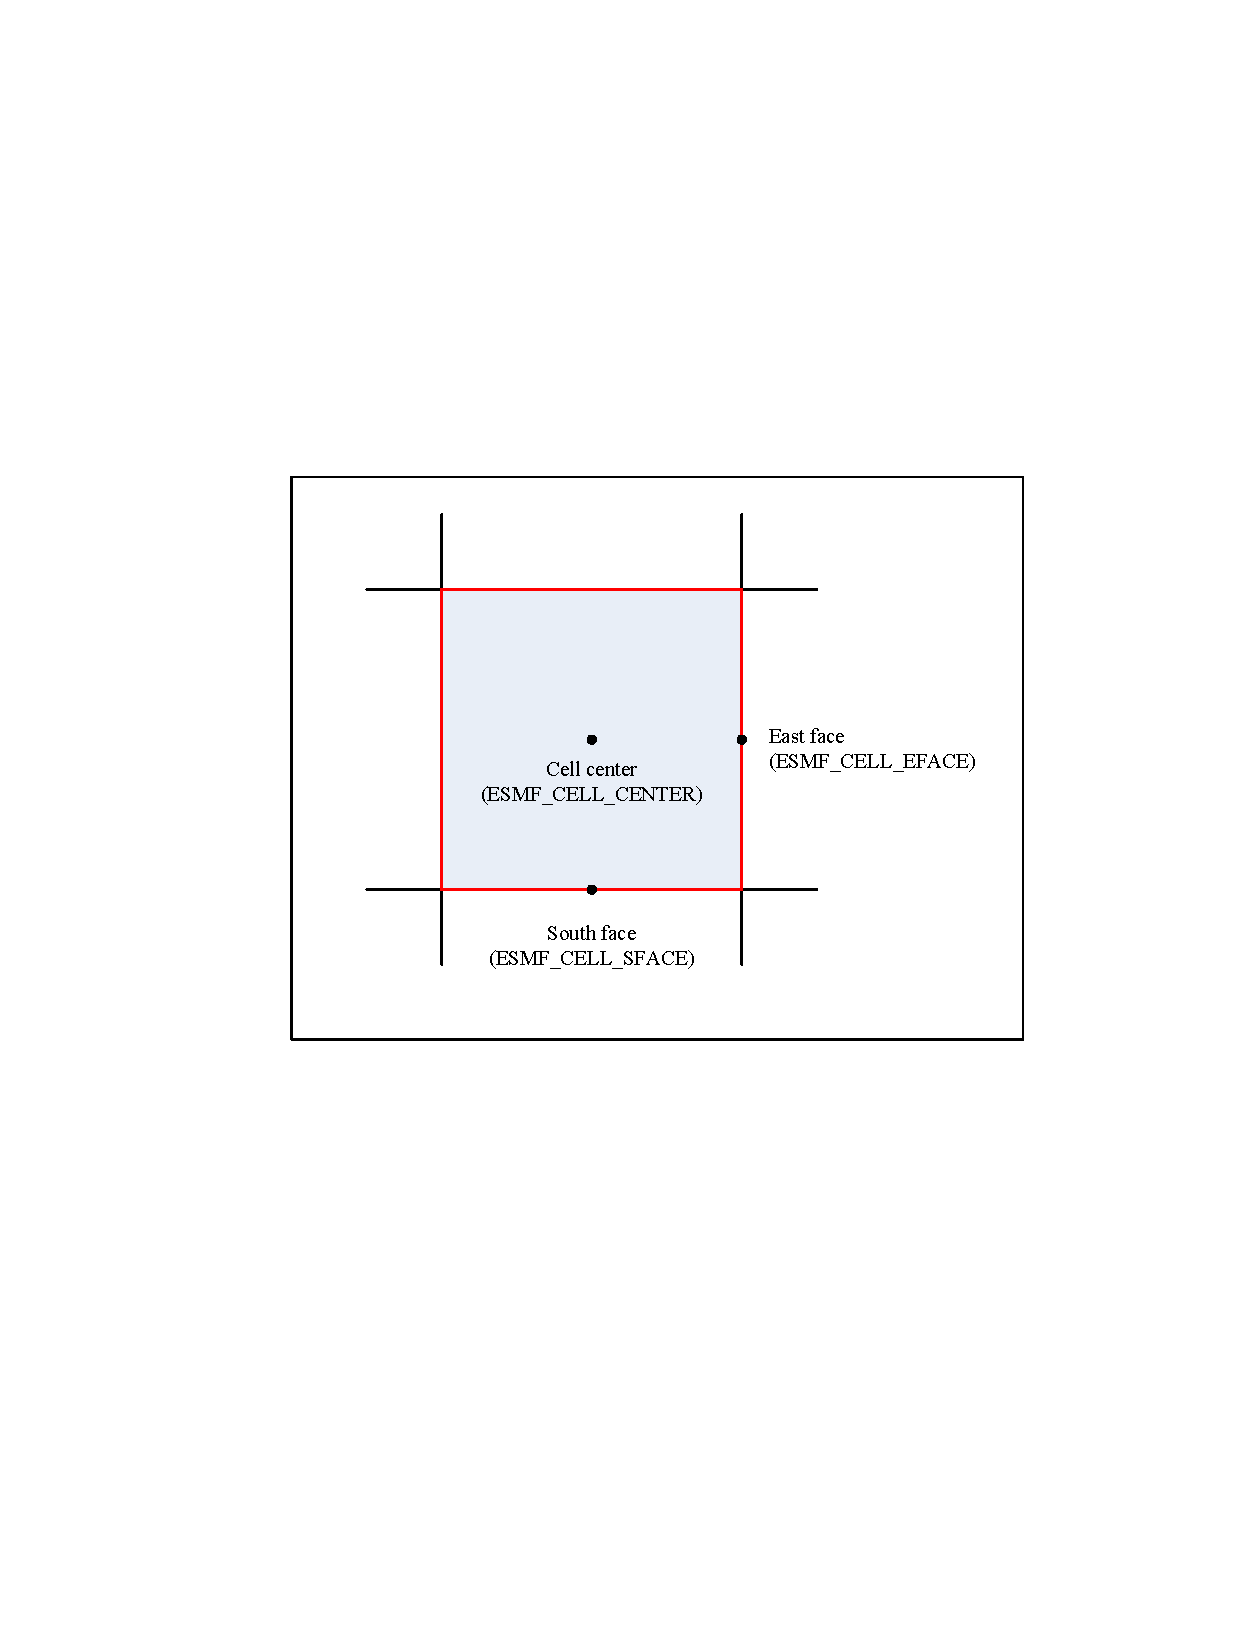
\includegraphics{ArakawaC_SE}}
% \end{figure}
% \end{center}

A vertical grid is also represented as one or more subGrids, each corresponding
to a specific relative location along the defined vertical axis.  The possible
% vertical relative locations are shown in Figure~\ref{fig:VertGridDataLocations}.

% DIAGFIX_BASELINE8
% \begin{center}
% \begin{figure}[h!tb]
% \caption{Possible vertical data locations for a representative computational
%          cell. }
% \label{fig:VertGridDataLocations}
% \scalebox{0.66}{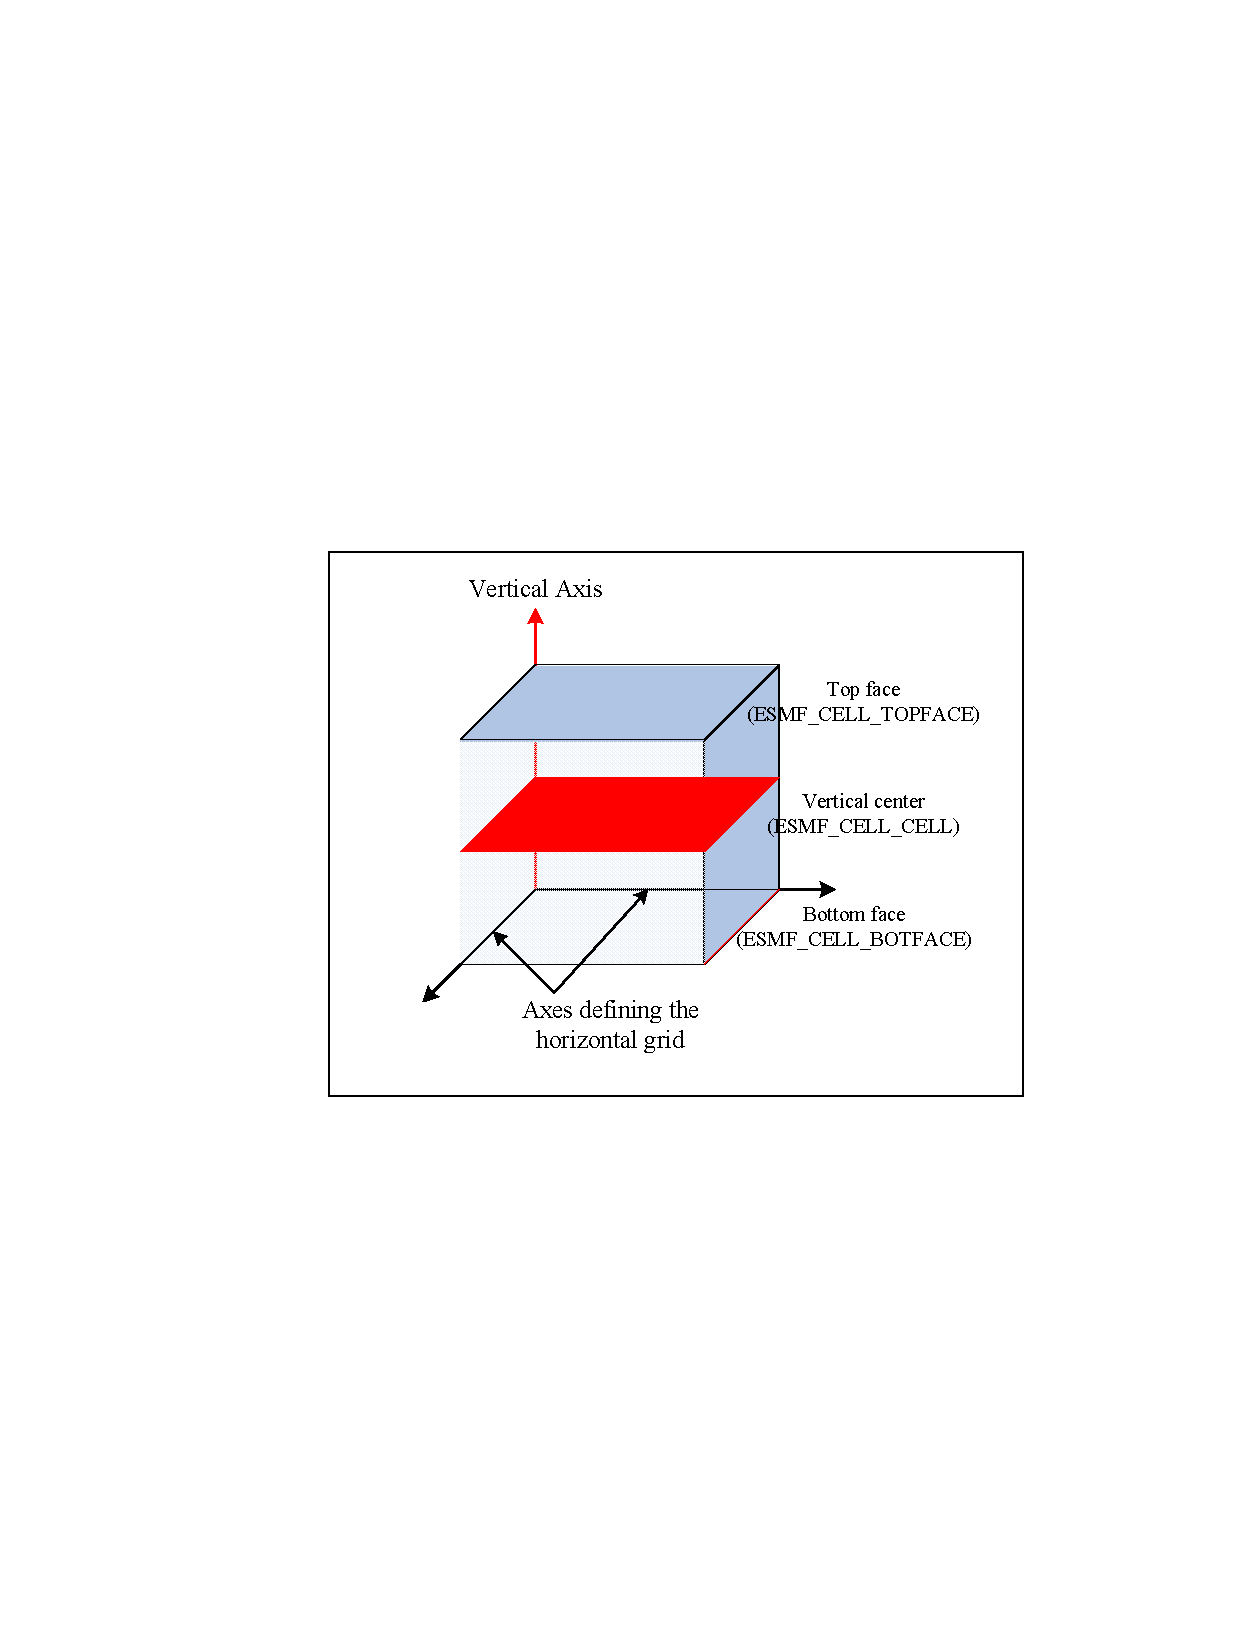
\includegraphics{VertGridDataLocations}}
% \end{figure}
% \end{center}

Note that the locations in the figure are represented by horizontal planes.  The
vertical relative location only defines the vertical coordinate of any point, and
does not restrict the horizontal coordinates.  This means that the horizontal and
vertical Rellocs are independent of each other and can be combined in any way.
For a complete list of implemented vertical staggerings and their corresponding
Rellocs, please see Section~\ref{sec:GridVertStagger}.

The staggering of the Grid limits the relative locations of any ESMF data 
class corresponding to it.  When an {\tt ESMF\_Field} is created, it must be
assigned to one (or more, in the case of a horizontal Grid with a vertical
subGrid) of the appropriate subGrids present in the {\tt ESMF\_Grid} from
which it is being created.  Continuing the example above, an {\tt ESMF\_Field}
created from a Grid with Arakawa C staggering would have to be defined at either
the cell center or one of the prescribed cell faces. 


\subsubsection{Grid Distribution}

The distribution (also referred to as decomposition) of the Grid on an
{\tt ESMF\_DELayout} determines the distribution as well for all related
ESMF data classes.  ESMF has currently implemented two different distribution
strategies: block and arbitrary.  In block distribution, logically rectangular
chunks of the global Grid are represented as local decomposition elements
% (DEs), as shown in Figure~\ref{fig:GridBlockDistribute}.

% DIAGFIX_BASELINE9
% \begin{center}
% \begin{figure}[h!tb]
% \caption{Illustration of Block Distribution of a Grid. }
% \label{fig:GridBlockDistribute}
% \scalebox{0.66}{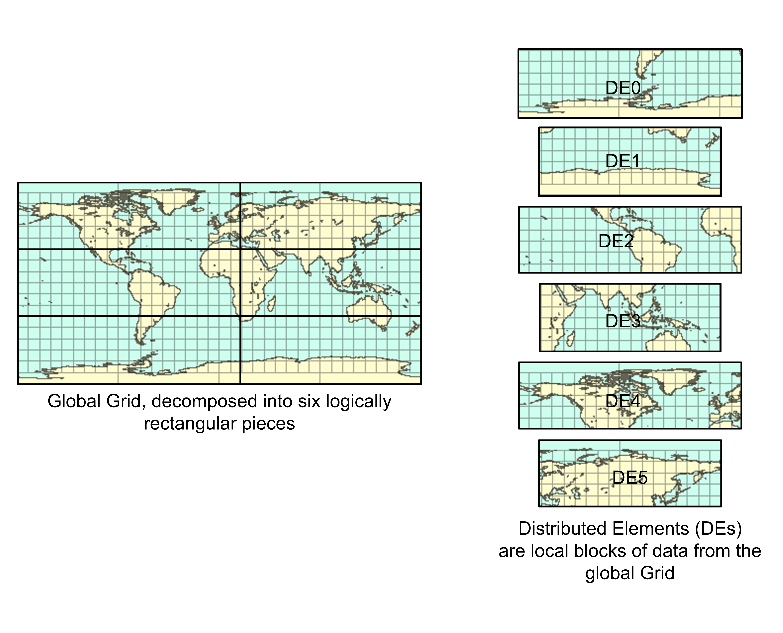
\includegraphics{GridBlockDistribution}}
% \end{figure}
% \end{center}

In this distribution method, some of the geometry and connectivity of the global
Grid are also true locally, in that most relative neighbor relationships are
maintained.  In arbitrary distribution, on the other hand, this is not
necessarily so, since the user specifies lists of individual points to
% be grouped as DEs, as shown in Figure~\ref{fig:GridArbitraryDistribute}.

% DIAGFIX_BASELINE10
% \begin{center}
% \begin{figure}[h!tb]
% \caption{Illustration of Arbitrary Distribution of a Grid. }
% \label{fig:GridArbitraryDistribute}
% \scalebox{0.66}{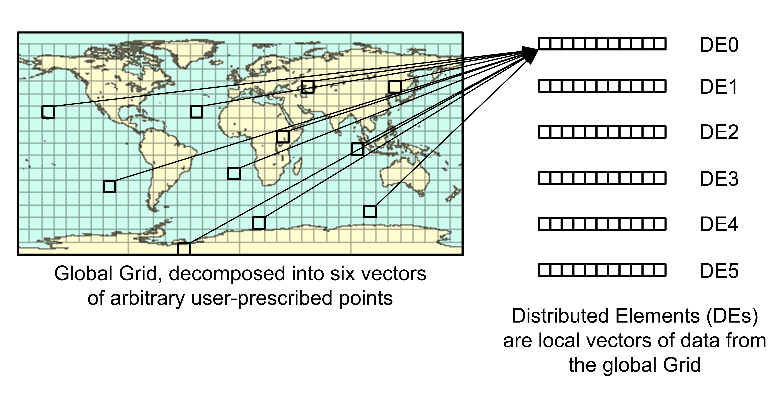
\includegraphics{GridArbitraryDistribution}}
% \end{figure}
% \end{center}

This method of distribution maintains local lists of cells without any sense
of their relationship to one another beyond their global index.  For that
reason, some higher level communication methods (like halo) would be 
inefficient for arbitrarily distributed Grids and their corresponding data
classes.  ESMF has implemented this distribution primarily to support 
components with column physics, which typically do not require much 
communication.  Currently for these objects ESMF only supports redistribution
between itself and a block distribution of the same global Grid to allow users
to move data from one representation to the other.
